\documentclass[a4paper,12pt]{article}
	%%%%%%%%%%%%%%%%%%%%%%%%%%%%%%%%%%%%%%%%%%%%%%%%%%%%%%%%%%%%%%%%%%%%%%%%%%%%%%%%%%%%%%%%%%%%%%%%%%%%%%%%%%%%%%%%%%%%%%%%%%%%%%%%%%%%%%%%%%%%%%%%%%%%%%%%%%%%%%%%%%%%%%%%%%%%%%%%%%%%%%%%%%%%%%%%%%%%%%%%%%%%%%%%%%%%%%%%%%%%%%%%%%%%%%%%%%%%%%%%%%%%%%%%%%%%
	\usepackage{eurosym}
	\usepackage{vmargin}
	\usepackage{amsmath}
	\usepackage{graphics}
	\usepackage{epsfig}
	\usepackage{subfigure}
	\usepackage{fancyhdr}
	\usepackage{listings}
	\usepackage{framed}
	\usepackage{graphicx}
	\usepackage{amsmath}
	\usepackage{chngpage}
	%\usepackage{bigints}
	
	
	\setcounter{MaxMatrixCols}{10}
	
	\begin{document}
		\Large
\section*{Components}
Bokeh is actually composed of two library components.

\begin{itemize}
	\item The first component is a JavaScript library, \texttt{BokehJS}, that runs in the browser. This library is responsible for all of the rendering and user interaction. Its input is a collection of declarative JSON objects that comprise a “scenegraph”. The objects in this scenegraph describe everything that BokehJS should handle: what plots and widgets are present and in what arrangement, what tools and renderers and axes the plots will have, etc. These JSON objects are converted into Backbone Models in the browser, and are rendered by corresponding Backbone Views.
	
	\item The second component is a library in Python (or other languages) that can generate the JSON described above. In the Python Bokeh library, this is accomplished at the lowest level by exposing a set of “model” classes that exactly mirror the set of Backbone Models that are created in the browser. These python model classes know how to validate their content and attributes, and also how to serialize themselves to JSON. 
	
\end{itemize}
\newpage
\section*{Interfaces}
\begin{figure}[h!]
	\centering
	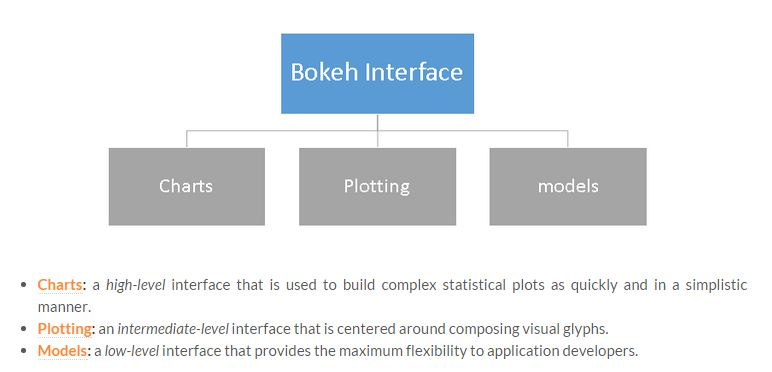
\includegraphics[width=1.1\linewidth]{images/00-Interfaces}
\end{figure}
\begin{itemize}
\item Bokeh is intended to be useful to data-scientists and domain experts, working at a very high level, as well as to application developers and software engineers, who may want more control or access to more sophisticated features. 
\item Because of this, Bokeh takes a layered approach and offers programming interfaces appropriate to different levels, as well as some compatibility interfaces to make use of existing code from other libraries. 

\item This section provides an overview of the different interfaces that are available to Bokeh users, as well as more context about the most important concepts central to the library. 
% If you’d like to jump right into plotting, go to Plotting with Basic Glyphs or Using High-level Charts.
\end{itemize}



%===================================================================================== %
\newpage

\section*{\texttt{bokeh.models}}

\begin{itemize}
\item All of the \textbf{\textit{low level}} models live in the low-level \texttt{bokeh.models} interface. \item Most of the models are very simple, usually consisting of a few property attributes and no methods. 
\item Model attributes can either be configured when the model is created, or later by setting attribute values on the model object. 

\end{itemize}

Here are some examples for a \texttt{Rect glyph} object:

\begin{framed}
\begin{verbatim}

# properties can be configured when a 
# model object is initialized
glyph = Rect(x="x", y="y2", 
     w=10, h=20, line_color=None)

# or by assigning values to attributes
# on the model later
glyph.fill_alpha = 0.5
glyph.fill_color = "navy"
\end{verbatim}
\end{framed}
\newpage
\begin{itemize}
\item These methods of configuration work in general for all Bokeh models. Because of that, and because all Bokeh interfaces ultimately produce collections of Bokeh models, styling and configuring plots and widgets is accomplished in basically the same way, regardless of which interface is used.

\item Using the \texttt{bokeh.models} interface provides complete control over how Bokeh plots and Bokeh widgets are put together and configured.\\ ( hence:  \textbf{\textit{Low Level}}) 
\item However, this provides no help with assembling the models in meaningful or correct ways. It is entirely up to developers to build the visualization piece by piece.

\item Most users will probably want to use one of the higher level interfaces described, unless they have specialized requirements that necessitate finer control. 
%For more information about the details of all Bokeh models, consult the Reference Guide.
\end{itemize}
\newpage
\section*{\texttt{bokeh.plotting}}
\begin{itemize}
\item Bokeh provides a \textbf{\textit{mid-level}} general purpose \texttt{bokeh.plotting} interface, which is similar in specificity to Matplotlib or Matlab style plotting interfaces.
\item It is centered around having users relate the visual glyphs they would like to have displayed to their data, and otherwise taking care of putting together plots with sensible default axes, grids, and tools. 
\item All the hard work to assemble the appropriate Bokeh Models to form a visualization that \textbf{\textit{BokehJS}} can render is handled automatically.

\item The main class in the \texttt{bokeh.plotting} interface is the \texttt{Figure} class. This is a subclass of the basic \texttt{Plot} model, that includes methods for easily adding different kinds of glyphs to a plot. 
\item Additionally it composes default axes, grids, and tools in the proper way without any extra effort. Typically, users will want to create \texttt{Figure} objects by using the \texttt{figure()} function.	
	\end{itemize}


%================================= %
\newpage
\noindent A prototypical example of the \texttt{bokeh.plotting} usage is show below, along with the resulting plot:

{
	\large
\begin{framed}
\begin{verbatim}
from bokeh.plotting import figure, output_file, show

# create a Figure object
p = figure(width=300, height=300,  
tools="pan,reset,save")

# add a Circle renderer to this figure
p.circle([1, 2.5, 3, 2], [2, 3, 1, 1.5], radius=0.3,
 alpha=0.5)

# specify how to output the plot(s)
output_file("output.html")

# display the figure
show(p)
\end{verbatim}
\end{framed}
}
\newpage
\begin{itemize}
\item The main observation is that the typical usage involves creating plots objects with the \texttt{figure()} function, then using the glyph methods like \texttt{Figure.circle} to add renderers for our data. 
\item We do not have to worry about configuring any axes or grids (although we can configure them if we need to), and specifying tools is done simply with the names of tools to add. 


% Note
\item Finally we use some output functions to display our plot. The output functions \texttt{output\_file()} and \texttt{show()}, etc. are defined in the \texttt{bokeh.io} module, but are also importable from \texttt{bokeh.plotting} for convenience.


\item There are many other possibilities: saving our plot instead of showing it, styling or removing the axes or grids, adding additional renderers, and laying out multiple plots together.
\end{itemize}
 

% The Plotting with Basic Glyphs section of this User Guide will walk through many more examples and common use cases of using the bokeh.plotting interface.

\newpage
\section*{\texttt{bokeh.charts}}
\begin{itemize}
\item Bokeh also provides a very high-level bokeh.charts interface for quickly creating statistical charts. 
\item As with \texttt{bokeh.plotting}, the main purpose of the interface is to help simplify the creation of Bokeh object graphs by encapsulating patterns of assembling Bokeh models. 
\item The \texttt{bokeh.charts} interface may also take the additional step of performing necessary statistical or data processing for the user. 

\item The interface presents functions for common, schematic statistical charts. \item Additionally, the chart functions can take care of automatically coloring and faceting based on group structure.
\end{itemize}

%================================================================== %
\newpage

\subsection*{Charts example}
The interface includes chart types such as: \texttt{Bar()}, \texttt{BoxPlot()}, \texttt{Histogram()}, \texttt{TimeSeries()}, and many others. 

One simple example using \texttt{Scatter()} is shown below:
{
	\begin{verbatim}
	
from bokeh.charts import Scatter, output_file, show

# prepare some data

from bokeh.sampledata.autompg import autompg as df

# create a scatter chart
p = Scatter(df, x='mpg', y='hp', color='cyl',
            title="MPG vs HP (colored by CYL)",
            legend='top_right',
            xlabel="Miles Per Gallon",
            ylabel="Horsepower")

# specify how to output the plot(s)
output_file("chart.html")

# display the figure
show(p)
\end{verbatim}

}

\newpage

Important to note is that the same output functions are used across different interfaces. As with \texttt{bokeh.plotting}, the output functions \texttt{output\_file()} and \texttt{show()}, etc. that are defined in bokeh.io, are also importable from \texttt{bokeh.charts} as a convenience.

\newpage
\section*{Other interfaces}
\begin{itemize}

\item Bokeh provides some level of Matplotlib compatibility, by using the third-party mplexporter library. 
\item Although it does not provide 100\% coverage of Matplotlib capabilities, it is still quite useful. 
\item For instance, in addition to many Matplotlib plots, it is often possible to convert plots created using the python Seaborn and \texttt{ggplot.py} libraries into Bokeh plots very easily. \item Here is a quick example that shows a Seaborn plot converted to a Bokeh plot with just one additional line of code:
\end{itemize}
\newpage

	\begin{verbatim}
import seaborn as sns

from bokeh import mpl
from bokeh.plotting import output_file, show

tips = sns.load_dataset("tips")

sns.set_style("whitegrid")

ax = sns.violinplot(x="day", y="total_bill", 
                    hue="sex",
                    data=tips, palette="Set2", 
                    split=True,
                    scale="count", inner="stick")

output_file("violin.html")

show(mpl.to_bokeh())
	
\end{verbatim}

\end{document}